\chapter{Soluções e solubilidade}\label{ch:g6:solutions-and-solubility}

Uma garrafa de água com gás é aberta: um chiado, e uma onda de bolhinhas
sobe do nada. Um segundo antes, a água parecia perfeitamente límpida, mas
havia um gás dissolvido nela o tempo todo. Os sólidos se dissolvem, os
líquidos se dissolvem, e os gases também se dissolvem --- mas nunca sem
limite. Este capítulo dá nome às partes de uma solução e mede quanto de
uma substância um líquido consegue conter.

\begin{recall}
Um sólido que \omterm{def:g2:mixing-and-dissolving:dissolve}{se dissolve} na água some da vista e deixa o líquido
límpido; o líquido límpido é uma solução, e o que foi dissolvido continua
nele (\cref{ch:g2:mixing-and-dissolving}). Uma solução é uma \omterm{def:g6:pure-substances-and-mixtures:homogeneous}{mistura
homogênea} de \omterm{def:g6:pure-substances-and-mixtures:species}{espécies químicas}
(\cref{ch:g6:pure-substances-and-mixtures}). Fazer a água evaporar
devolve o sólido dissolvido (\cref{ch:g3:separating-mixtures}).
\end{recall}

\begin{omfigure}
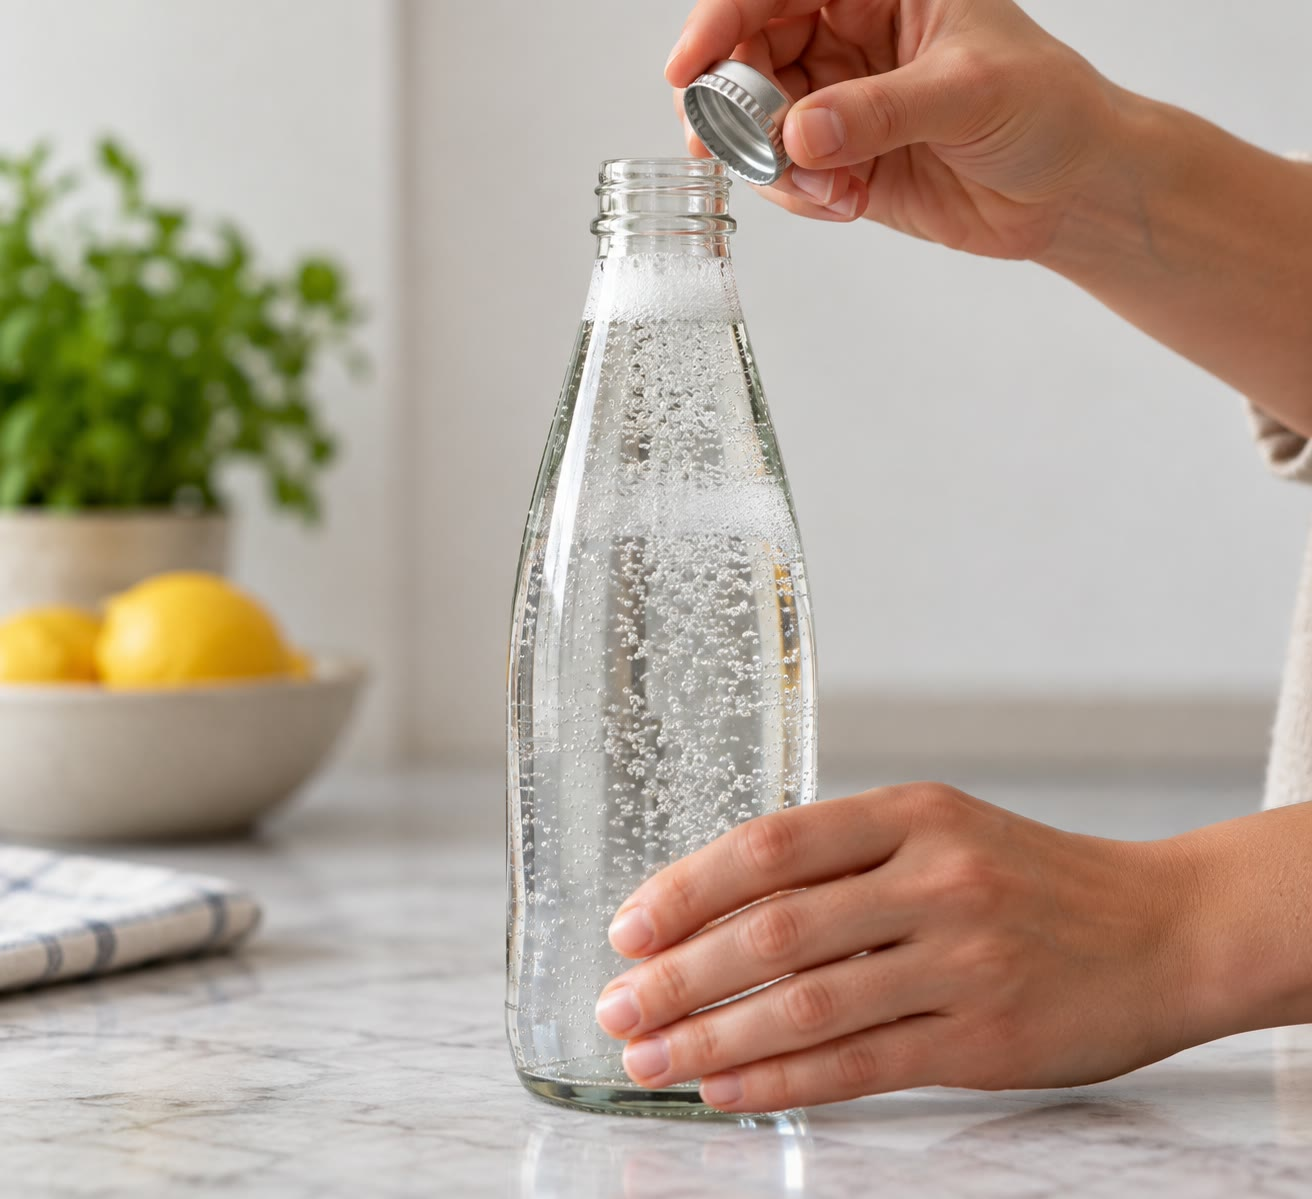
\includegraphics[width=0.5\linewidth]{images/book1/ai/g6-fizzy-water.jpg}

{\small Abrindo uma garrafa de água com gás: o gás dissolvido sai em
forma de bolhas.}
\end{omfigure}

\section{Soluto e solvente}

\begin{definition}[Soluto, solvente, solução aquosa]\label{def:g6:solutions-and-solubility:solute}
Numa solução, a substância que \omterm{def:g2:mixing-and-dissolving:dissolve}{se dissolve} é o
\emph{soluto}\index{soluto}, e o líquido em que ela \omterm{def:g2:mixing-and-dissolving:dissolve}{se dissolve} é o
\emph{solvente}\index{solvente}. Quando o solvente é a água, a solução é
uma \emph{solução aquosa}\index{solucao aquosa@solução aquosa}.
\end{definition}

\begin{example}[Outros solventes além da água]\label{ex:g6:solutions-and-solubility:solvents}
A água é o \omterm{def:g6:solutions-and-solubility:solute}{solvente} mais comum, mas não o único. O esmalte de unha não
\omterm{def:g2:mixing-and-dissolving:dissolve}{se dissolve} na água; ele \omterm{def:g2:mixing-and-dissolving:dissolve}{se dissolve} na propanona (acetona), o \omterm{def:g6:solutions-and-solubility:solute}{solvente}
do removedor de esmalte. A graxa e a tinta a óleo se dissolvem na
aguarrás. Muitos remédios são dissolvidos em etanol. Uma solução pode
ter vários \omterm{def:g6:solutions-and-solubility:solute}{solutos}: a água do mar contém sal dissolvido e muitas outras
substâncias.
\end{example}

\begin{safety}{\ghs{GHS02}\ghs{GHS07}}
% ledger: ghs:acetone
Propanona (acetona): líquido e vapor altamente inflamáveis (GHS02); ela
irrita os olhos e o seu vapor pode provocar sonolência ou tontura
(GHS07). Ela é usada num local ventilado, longe de qualquer chama.
\end{safety}

\begin{proposition}[As massas se somam]\label{prop:g6:solutions-and-solubility:mass}
A massa de uma solução é a massa do \omterm{def:g6:solutions-and-solubility:solute}{solvente} mais a massa do \omterm{def:g6:solutions-and-solubility:solute}{soluto}
dissolvido: nada se perde quando um sólido \omterm{def:g2:mixing-and-dissolving:dissolve}{se dissolve}, mesmo que ele não
possa mais ser visto.
\end{proposition}

\begin{omfigure}
\begin{tikzpicture}[font=\small, scale=1.15]
  \pic[transform shape] at (0,0) {balance};
  \pic[transform shape] at (0,0.8) {beaker={0.5}{omWater!80}};
  \node[anchor=north, align=center] at (0,-0.1) {\qty{100}{g} de água};
  \node at (1.85,1.3) {$+$};
  \pic[transform shape] at (3.5,0) {balance};
  \fill[white, draw=black!45] (3.0,0.8) rectangle (4.0,0.9);
  \fill[white, draw=black!45] (3.15,0.9) -- (3.85,0.9) -- (3.5,1.2) -- cycle;
  \node[anchor=north, align=center] at (3.5,-0.1) {\qty{10}{g} de açúcar};
  \draw[->, thick, omProp] (4.9,1.2) -- (6.0,1.2) node[midway, above, text=black]
    {mexer};
  \pic[transform shape] at (7.4,0) {balance};
  \pic[transform shape] at (7.4,0.8) {beaker={0.52}{omWater!80}};
  \node[anchor=north, align=center] at (7.4,-0.1) {\qty{110}{g} de água com açúcar};
\end{tikzpicture}

{\small \omterm{def:g2:mixing-and-dissolving:dissolve}{Dissolver} \qty{10}{g} de açúcar em \qty{100}{g} de água dá
\qty{110}{g} de solução (a massa do béquer não é contada).}
\end{omfigure}

\section{Saturação e solubilidade}

\begin{definition}[Solução saturada]\label{def:g6:solutions-and-solubility:saturated}
Uma solução é uma \emph{solução saturada}\index{solucao saturada@solução saturada} quando
ela não consegue \omterm{def:g2:mixing-and-dissolving:dissolve}{dissolver} mais nada do seu \omterm{def:g6:solutions-and-solubility:solute}{soluto}: todo \omterm{def:g6:solutions-and-solubility:solute}{soluto}
acrescentado fica no fundo, sem se \omterm{def:g2:mixing-and-dissolving:dissolve}{dissolver}, por mais que a gente mexa.
\end{definition}

\begin{definition}[Solubilidade]\label{def:g6:solutions-and-solubility:solubility}
A \emph{solubilidade}\index{solubilidade} de um \omterm{def:g6:solutions-and-solubility:solute}{soluto} num \omterm{def:g6:solutions-and-solubility:solute}{solvente} é a
maior massa de \omterm{def:g6:solutions-and-solubility:solute}{soluto} que uma dada quantidade de \omterm{def:g6:solutions-and-solubility:solute}{solvente} consegue
\omterm{def:g2:mixing-and-dissolving:dissolve}{dissolver}, a uma dada temperatura. Para um sólido na água, ela muitas
vezes é dada em gramas por litro (ou por quilograma) de água.
\end{definition}

\begin{proposition}[Algumas solubilidades na água]\label{prop:g6:solutions-and-solubility:values}
% ledger: sol:NaCl, sol:sucrose, sol:CO2, sol:O2 (O2: 31 mL/L, 31/24.0 x 32 = 0.041 g/L at 20 C)
As \omterm{def:g6:solutions-and-solubility:solubility}{solubilidades} medidas na água são extremamente diferentes:
\begin{center}
\small
\begin{tabular}{lll}
\hline
\omterm{def:g6:solutions-and-solubility:solute}{soluto} & \omterm{def:g6:solutions-and-solubility:solubility}{solubilidade} na água & condições \\
\hline
açúcar (sacarose) & cerca de \qty{2000}{g} por litro de água & temperatura ambiente \\
sal (cloreto de sódio) & \qty{360}{g} por quilograma de água & \qty{25}{\celsius} \\
dióxido de carbono & cerca de \qty{1.5}{g} por litro & \qty{25}{\celsius}, sob o gás \\
oxigênio & cerca de \qty{0.04}{g} por litro & \qty{20}{\celsius}, sob o gás \\
areia, giz & praticamente nada & --- \\
\hline
\end{tabular}
\end{center}
Um litro de água consegue \omterm{def:g2:mixing-and-dissolving:dissolve}{dissolver} mais do que a sua própria massa de
açúcar, mas nem meio grama de oxigênio.
\end{proposition}

\begin{method}[Vai dissolver tudo?]\label{met:g6:solutions-and-solubility:will-it}
Para saber se uma massa $m$ de \omterm{def:g6:solutions-and-solubility:solute}{soluto} \omterm{def:g2:mixing-and-dissolving:dissolve}{se dissolve} completamente num
volume de água:
\begin{enumerate}
  \item procure a \omterm{def:g6:solutions-and-solubility:solubility}{solubilidade} do \omterm{def:g6:solutions-and-solubility:solute}{soluto} (em g por litro de água);
  \item calcule a maior massa que esse volume de água consegue \omterm{def:g2:mixing-and-dissolving:dissolve}{dissolver};
  \item compare com $m$: se $m$ for menor, tudo \omterm{def:g2:mixing-and-dissolving:dissolve}{se dissolve}; se $m$ for
        maior, a solução fica saturada e o resto fica no fundo.
\end{enumerate}
\end{method}

\begin{example}[Sal num copo]\label{ex:g6:solutions-and-solubility:glass}
% ledger: sol:NaCl
\qty{50}{g} de sal conseguem se \omterm{def:g2:mixing-and-dissolving:dissolve}{dissolver} em \qty{200}{mL} de água
(cerca de \qty{200}{g})? Um quilograma de água dissolve no máximo
\qty{360}{g} de sal, então \qty{200}{g} de água dissolvem no máximo
$360 \times
\frac{200}{1000} = \qty{72}{g}$. Como $50 < 72$, todo o sal \omterm{def:g2:mixing-and-dissolving:dissolve}{se
dissolve}.
\end{example}

\begin{omfigure}
\begin{tikzpicture}[font=\small, scale=1.15]
  \pic[transform shape] at (0,0) {beaker={0.6}{omWater!80}};
  \node[anchor=north, align=center] at (0,-0.15) {pouco sal:\\ tudo dissolvido};
  \pic[transform shape] at (3.2,0) {beaker={0.6}{omWater!80}};
  \node[anchor=north, align=center] at (3.2,-0.15) {mais sal:\\ no limite da saturação};
  \pic[transform shape] at (6.4,0) {beaker={0.6}{omWater!80}};
  \fill[black!12, draw=black!50] (5.7,0) -- (7.1,0) -- (6.9,0.2) -- (5.9,0.2) -- cycle;
  \foreach \x in {5.85,6.05,6.25,6.45,6.65,6.85} \fill[black!45] (\x,0.09) circle (0.03);
  \node[anchor=north, align=center] at (6.4,-0.15) {sal demais:\\ o resto não se dissolve};
\end{tikzpicture}

{\small Acrescentando cada vez mais sal à mesma água. Depois que a
solução fica saturada, o sal a mais fica no fundo.}
\end{omfigure}

\begin{inthelab}[Saturar água salgada]
O professor acrescenta sal a \qty{100}{mL} de água, uma colherada de
cada vez, mexendo bem depois de cada uma. As primeiras colheradas
desaparecem; depois, uma colherada já não \omterm{def:g2:mixing-and-dissolving:dissolve}{se dissolve} completamente e
grãos brancos ficam no fundo: a solução está saturada. Pesando o sal
usado, vê-se que cerca de \qty{36}{g} se dissolveram.
\end{inthelab}

\section{Líquidos miscíveis e imiscíveis}

\begin{definition}[Líquidos miscíveis e imiscíveis]\label{def:g6:solutions-and-solubility:miscible}
Dois líquidos são \emph{miscíveis}\index{miscivel@miscível} quando, \omterm{def:g2:mixing-and-dissolving:mix}{misturados},
dão um único líquido homogêneo. Eles são
\emph{imiscíveis}\index{imiscivel@imiscível} quando se separam em duas camadas, o
mais leve em cima.
\end{definition}

\begin{example}[Água com etanol, água com óleo]\label{ex:g6:solutions-and-solubility:liquids}
A água e o etanol são \omterm{def:g6:solutions-and-solubility:miscible}{miscíveis}: sacudidos juntos, eles dão um único
líquido límpido. A água e o óleo são \omterm{def:g6:solutions-and-solubility:miscible}{imiscíveis}: por mais que sejam
sacudidos, o óleo volta para cima e flutua sobre a água numa camada
separada. Num vidro de molho de salada, o óleo flutua acima do vinagre,
que é principalmente água.
\end{example}

\begin{omfigure}
\begin{tikzpicture}[font=\small, scale=1.3]
  \pic[transform shape] at (0,0) {testtube={0.6}{omWater!80}};
  \node[anchor=north, align=center] at (0,-0.15) {água + etanol:\\ uma camada};
  \pic[transform shape] at (3,0) {testtube={0.65}{yellow!55!orange!60}};
  \begin{scope}
    \clip (2.75,3) -- (2.75,0.25) arc[start angle=180, end angle=360, radius=0.25]
      -- (3.25,3) -- cycle;
    \fill[omWater!80] (2.7,0) rectangle (3.3,1.1);
  \end{scope}
  \draw[omGlass, line width=0.7pt] (2.75,3) -- (2.75,0.25) arc[start angle=180,
    end angle=360, radius=0.25] -- (3.25,3);
  \draw[<-, omProp, thick] (3.3,1.55) -- (4.1,1.75) node[right, text=black] {óleo};
  \draw[<-, omProp, thick] (3.3,0.6) -- (4.1,0.6) node[right, text=black] {água};
  \node[anchor=north, align=center] at (3,-0.15) {água + óleo:\\ duas camadas};
\end{tikzpicture}

{\small Líquidos \omterm{def:g6:solutions-and-solubility:miscible}{miscíveis} dão uma camada; líquidos \omterm{def:g6:solutions-and-solubility:miscible}{imiscíveis} dão duas.}
\end{omfigure}

\begin{omfigure}
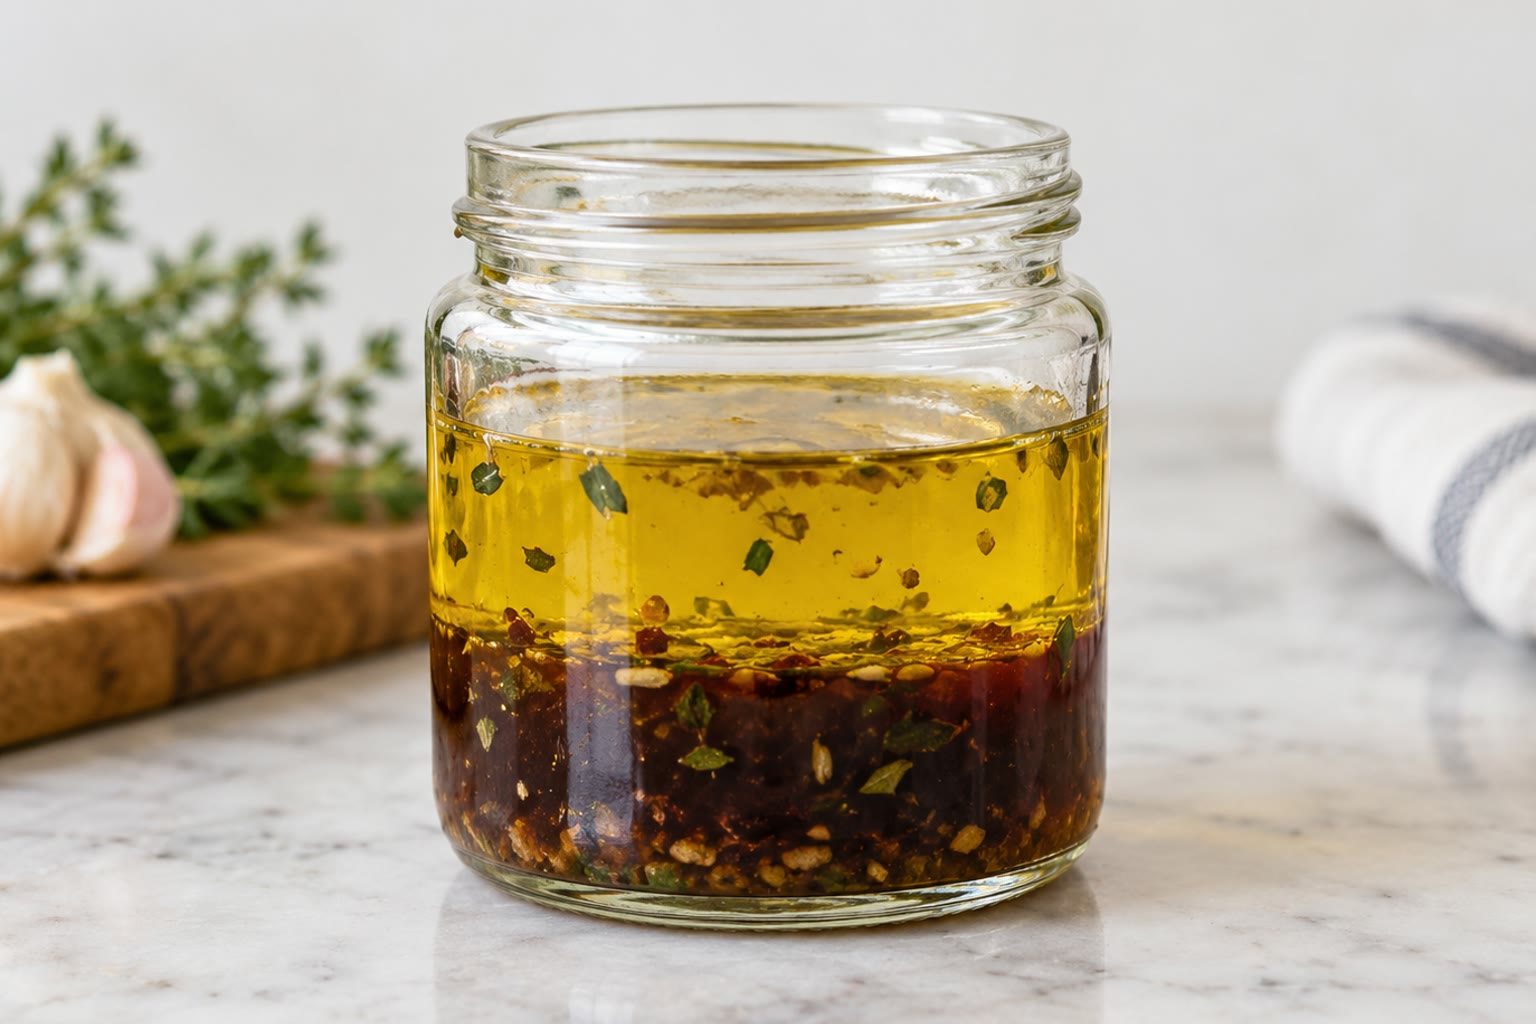
\includegraphics[width=0.45\linewidth]{images/book1/ai/g6-vinaigrette.jpg}

{\small Molho de salada: o óleo e o vinagre são \omterm{def:g6:solutions-and-solubility:miscible}{imiscíveis}.}
\end{omfigure}

\section{Os gases também se dissolvem}

\begin{proposition}[Gases dissolvidos]\label{prop:g6:solutions-and-solubility:gases}
Os gases se dissolvem na água, um pouco. As bebidas com gás são feitas
dissolvendo dióxido de carbono nelas sob pressão, numa garrafa fechada;
quando a garrafa é aberta, parte do gás volta a sair em forma de bolhas.
A água em contato com o \omterm{def:g4:air-a-mixture-of-gases:air}{ar} contém um pouco de oxigênio dissolvido, que
os peixes absorvem pelas brânquias. Um gás \omterm{def:g2:mixing-and-dissolving:dissolve}{se dissolve} menos na água
morna do que na água fria: um refrigerante quente perde o gás mais
depressa.
\end{proposition}

\begin{example}[Os oceanos e o dióxido de carbono]\label{ex:g6:solutions-and-solubility:oceans}
Os oceanos estão em contato com o \omterm{def:g4:air-a-mixture-of-gases:air}{ar} em dois terços da superfície da
Terra. O dióxido de carbono do \omterm{def:g4:air-a-mixture-of-gases:air}{ar} \omterm{def:g2:mixing-and-dissolving:dissolve}{se dissolve} neles, e assim os oceanos
absorvem uma parte do dióxido de carbono que as pessoas lançam no \omterm{def:g4:air-a-mixture-of-gases:air}{ar}.
\end{example}

\begin{omfigure}
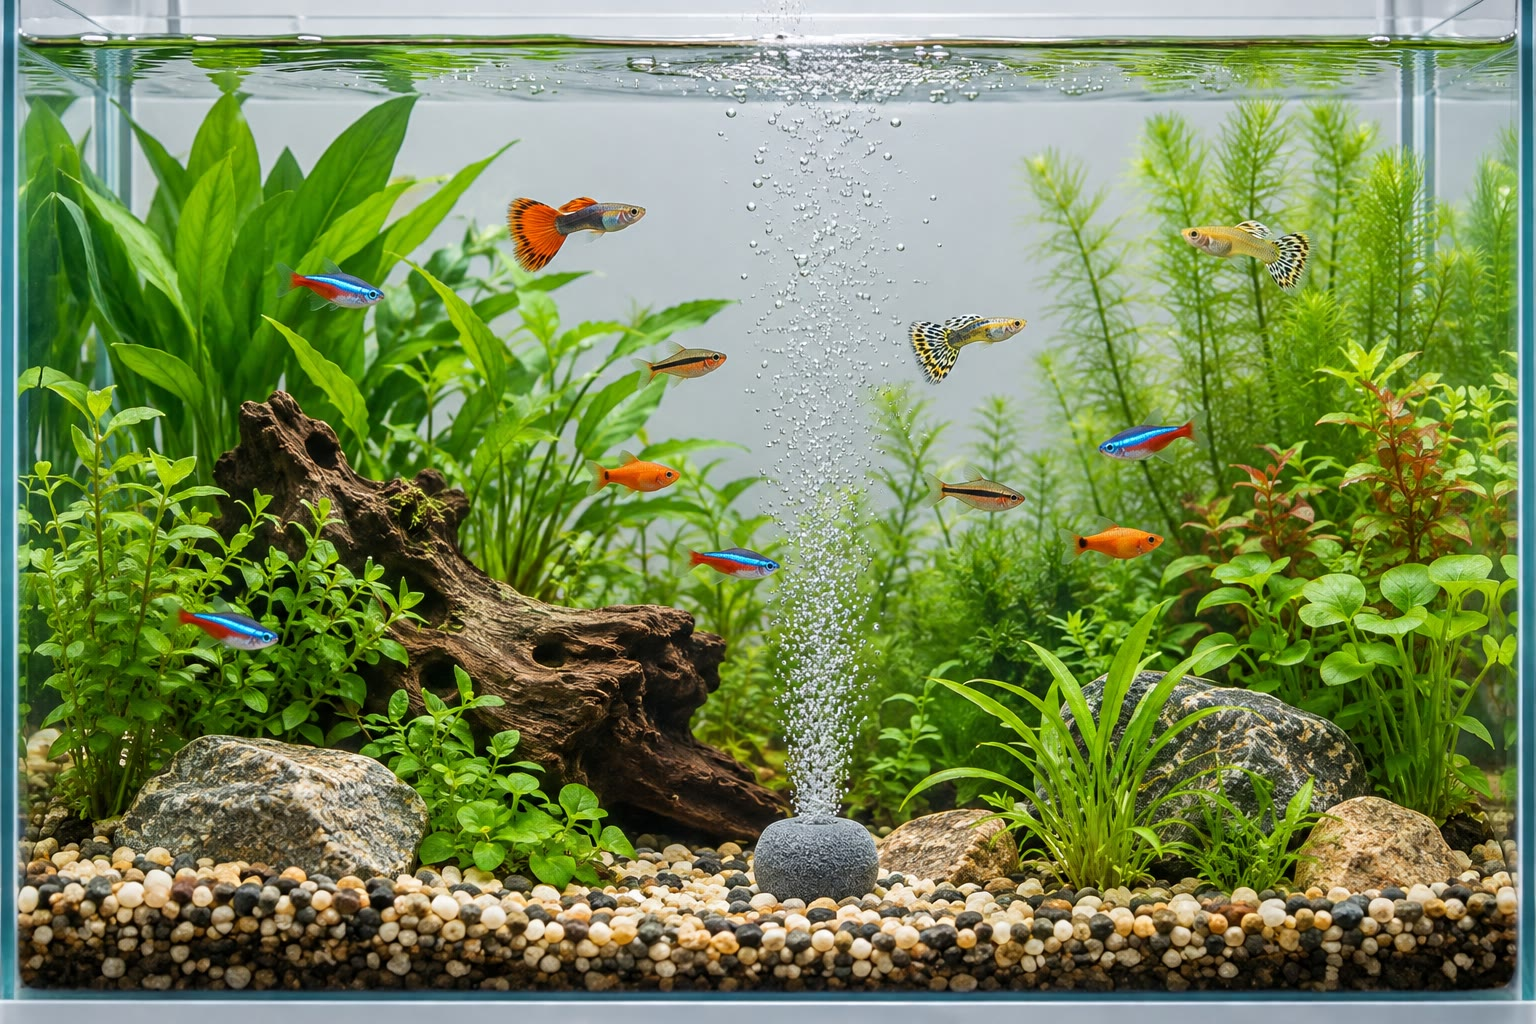
\includegraphics[width=0.5\linewidth]{images/book1/ai/g6-fish-tank.jpg}

{\small Um aquário: as bolhas de \omterm{def:g4:air-a-mixture-of-gases:air}{ar} mantêm a água abastecida de oxigênio
dissolvido para os peixes.}
\end{omfigure}

\section{Exercícios}

\begin{exercise}[$\star$]\label{exo:g6:solutions-and-solubility:1}
Na água com açúcar, diga qual é o \omterm{def:g6:solutions-and-solubility:solute}{soluto} e qual é o \omterm{def:g6:solutions-and-solubility:solute}{solvente}. É uma
\omterm{def:g6:solutions-and-solubility:solute}{solução aquosa}?
\end{exercise}

\begin{exercise}[$\star$]\label{exo:g6:solutions-and-solubility:2}
O que é uma \omterm{def:g6:solutions-and-solubility:saturated}{solução saturada}? Como dá para ver que uma solução está
saturada?
\end{exercise}

\begin{exercise}[$\star$]\label{exo:g6:solutions-and-solubility:3}
Dissolvem-se \qty{20}{g} de sal em \qty{250}{g} de água. Qual é a massa
da solução?
\end{exercise}

\begin{exercise}[$\star$]\label{exo:g6:solutions-and-solubility:4}
\omterm{def:g6:solutions-and-solubility:miscible}{Miscível} ou \omterm{def:g6:solutions-and-solubility:miscible}{imiscível} com a água: etanol, óleo de cozinha, vinagre?
\end{exercise}

\begin{exercise}[$\star$]\label{exo:g6:solutions-and-solubility:5}
Diga qual é o \omterm{def:g6:solutions-and-solubility:solute}{solvente} do removedor de esmalte e dê o significado dos
seus dois pictogramas.
\end{exercise}

\begin{exercise}[$\star\star$]\label{exo:g6:solutions-and-solubility:6}
Usando a \omterm{def:g6:solutions-and-solubility:solubility}{solubilidade} do sal, encontre a maior massa de sal que
\qty{500}{g} de água conseguem \omterm{def:g2:mixing-and-dissolving:dissolve}{dissolver} a \qty{25}{\celsius}.
\end{exercise}

\begin{exercise}[$\star\star$]\label{exo:g6:solutions-and-solubility:7}
Mexem-se \qty{80}{g} de sal em \qty{200}{g} de água a
\qty{25}{\celsius}. Tudo \omterm{def:g2:mixing-and-dissolving:dissolve}{se dissolve}? Se não, que massa fica no fundo?
\end{exercise}

\begin{exercise}[$\star\star$]\label{exo:g6:solutions-and-solubility:8}
Dissolvem-se \qty{25}{g} de açúcar em \qty{225}{g} de água. Que
porcentagem da massa da solução é açúcar?
\end{exercise}

\begin{exercise}[$\star\star$]\label{exo:g6:solutions-and-solubility:9}
Olhe a figura dos três béqueres de água salgada. Em que béquer ainda
poderia se \omterm{def:g2:mixing-and-dissolving:dissolve}{dissolver} mais sal?
\end{exercise}

\begin{exercise}[$\star\star$]\label{exo:g6:solutions-and-solubility:10}
Por que uma garrafa de água com gás borbulha quando é aberta, e não
antes?
\end{exercise}

\begin{exercise}[$\star\star\star$]\label{exo:g6:solutions-and-solubility:11}
Um litro de água consegue \omterm{def:g2:mixing-and-dissolving:dissolve}{dissolver} cerca de \qty{2000}{g} de açúcar,
mas só cerca de \qty{0.04}{g} de oxigênio. Quantas vezes mais açúcar do
que oxigênio é isso?
\end{exercise}

\begin{exercise}[$\star\star\star$]\label{exo:g6:solutions-and-solubility:12}
No verão, a água de um lago esquenta e os peixes sobem até a superfície
para engolir \omterm{def:g4:air-a-mixture-of-gases:air}{ar}. Use este capítulo para explicar por quê.
\end{exercise}

\section{Problema: a salmoura do queijeiro}

\begin{problem}[{Problema de fim de semana --- um banho de água
saturada de sal para queijos, e o que o calor do verão faz com ele}]
\label{pb:g6:solutions-and-solubility:1}
% ledger: sol:NaCl (360 g per kg of water; 1 L of water taken as 1 kg)
Muitos queijos ficam de molho por algumas horas num banho de salmoura:
água saturada de sal. Um queijeiro enche um tanque com \qty{20}{L} de
água (\qty{20}{kg}) e acrescenta sal até que um pouco fique sem se
\omterm{def:g2:mixing-and-dissolving:dissolve}{dissolver} no fundo. Tome a \omterm{def:g6:solutions-and-solubility:solubility}{solubilidade} do sal como \qty{360}{g} por
quilograma de água.

\medskip
\noindent\textbf{Parte I --- As palavras.}
\begin{enumerate}
  \item Na salmoura, qual é o \omterm{def:g6:solutions-and-solubility:solute}{soluto} e qual é o \omterm{def:g6:solutions-and-solubility:solute}{solvente}?
  \item O que ``saturada'' quer dizer para a salmoura?
  \item Por que o queijeiro acrescenta sal até que um pouco fique no
        fundo?
\end{enumerate}

\medskip
\noindent\textbf{Parte II --- Preparar a salmoura.}
\begin{enumerate}[resume]
  \item Que massa de sal \omterm{def:g2:mixing-and-dissolving:dissolve}{se dissolve} nos \qty{20}{kg} de água?
  \item Qual é a massa da salmoura (sem o sal não dissolvido)?
  \item Que porcentagem da massa da salmoura é sal? Arredonde para o
        número inteiro mais próximo.
  \item Num certo dia, só são acrescentados \qty{5}{kg} de sal. A
        salmoura está saturada? Quanto sal a mais ela ainda poderia
        \omterm{def:g2:mixing-and-dissolving:dissolve}{dissolver}?
\end{enumerate}

\medskip
\noindent\textbf{Parte III --- Um verão quente.}
Durante uma semana quente, \qty{5}{L} (\qty{5}{kg}) de água \omterm{def:g3:separating-mixtures:evaporate}{evaporam} da
salmoura saturada da Parte II, e nenhum sal se perde.
\begin{enumerate}[resume]
  \item Quanta água sobra no tanque?
  \item Que massa de sal essa água ainda consegue manter dissolvida?
  \item O que acontece com o sal que a água restante não consegue manter
        dissolvido?
  \item Como o queijeiro pode ver, olhando, que isso aconteceu?
  \item Calcule a massa de sal que cristalizou no fundo do tanque.
\end{enumerate}
\end{problem}
